\documentclass[journal,hidelinks]{IEEEtran}
\usepackage[utf8]{inputenc}
\usepackage[
  pdftitle={Assignment \#3},
  pdfauthor={Andrei Purcarus},
  pdfsubject={ECSE-534 -- Analog Microelectronics}
]{hyperref}
\usepackage{graphicx}
\usepackage[all]{hypcap}
\usepackage{cleveref}
\usepackage{indentfirst}
\usepackage[per-mode=symbol]{siunitx}

\title{ECSE-534 \\ Analog Microelectronics \\ Assignment \#3}
\author{Andrei~Purcarus,~260631911,~\IEEEmembership{McGill~University} \\ \href{mailto:andrei.purcaruscraciun@mail.mcgill.ca}{andrei.purcaruscraciun@mail.mcgill.ca}}

\begin{document}
\sloppy

\maketitle

\begin{abstract}

The layout for the CMOS amplifier designed in Assignment \#2 was performed using Cadence. The performance of the amplifier with layout parasitics extracted was then compared to the performance of the amplifier using only the schematic models. No significant difference between the two was found, with the largest change being a small degradation of the step response due to the additional capacitances at each node. In particular, the amplifier was found to still meet all the specifications required of it in Assignment \#2 after layout.

\end{abstract}

\section{Introduction}

\IEEEPARstart{T}{his} report follows the layout of the amplifier designed in Assignment \#2 using a 0.13 micron process from IBM. We used Cadence and Virtuoso to lay out the amplifier, and we used Analog Environment to perform simulation using said process. In the original specifications, the amplifier was required to meet the following specs:
\begin{itemize}
\item DC gain $\ge$ $\SI{60}{\deci\bel}$.
\item Amplifier poles at approx. $\SI{10}{\kilo\hertz}$ and $\SI{100}{\mega\hertz}$. Others above this.
\item Output voltage swings of at least $\SI{50}{\percent}$ of the supply full scale with a distortion less than $\SI{0.2}{\percent}$ in a unity-gain configuration.
\item Input-referred PSD Noise Voltage less than $\SI{100}{\nano\volt\per\sqrt{\hertz}}$ at $\SI{1}{\mega\hertz}$.
\item Static power dissipation less than $\SI{200}{\micro\watt}$.
\end{itemize}

In addition, we were assigned a supply voltage of $\SI{1.2}{\volt}$, a common mode input voltage of $\SI{0.5}{\volt}$, and a load capacitance of $\SI{0.5}{\pico\farad}$.

To perform the given task, we first redesigned the amplifier from Assignment \#2 to be better suited for layout. Then, we performed the layout, taking into consideration transistor matching and signal path length. Finally, we extracted the parasitics from the layout and compared the resulting performance of the amplifier to that of the amplifier with just the schematic models.

\section{Layout-Ready Design}

First, we redesigned the amplifier to be more layout friendly. We did this in order to facilitate the use of techniques for transistor matching in the layout process, such as using a common centroid topology. We made all transistors integer multiples of a unit size transistor in order to reduce component parameter variations. We also ensured that every transistor pair that performs the same function has an even multiplicity in order to better match them using a common centroid topology. We also tweaked the transistor widths to meet the specs in the original assignment after these modifications. The final layout-ready amplifier is shown in \Cref{fig:amplifier}. The transistor dimensions are given in \Cref{tab:dim-final-1,tab:dim-final-2}. We also selected $R_b = \SI{56}{\kilo\ohm}$, $C_C = \SI{0.33}{\pico\farad}$, and $R_C = \SI{7.2}{\kilo\ohm}$.

\begin{figure*}[!htb]
  \centering
  \includegraphics[width=\textwidth]{schematics/amplifier.pdf}
  \caption{A schematic of the complete layout-ready amplifier.}
  \label{fig:amplifier}
\end{figure*}

\begin{table}[!htb]
  \centering
  \caption{Final transistor dimensions (Part 1).}
  \label{tab:dim-final-1}
  \resizebox{\columnwidth}{!}{\begin{tabular}{|c|c|c|c|c|c|c|c|c|c|c|}
    \hline
     & T1 & T2 & T3 & T4 & T5 & T6 & T7 & T8 & T9 & T10 \\ \hline
    W (\SI{}{\micro\meter}) & 4.0 & 4.0 & 0.8 & 0.8 & 2.0 & 2.0 & 2.0 & 2.0 & 12 & 32 \\ \hline
    L (\SI{}{\micro\meter}) & 0.4 & 0.4 & 0.4 & 0.4 & 0.4 & 0.4 & 0.4 & 0.4 & 0.4 & 0.4 \\ \hline
  \end{tabular}}
\end{table}

\begin{table}[!htb]
  \centering
  \caption{Final transistor dimensions (Part 2).}
  \label{tab:dim-final-2}
  \resizebox{\columnwidth}{!}{\begin{tabular}{|c|c|c|c|c|c|c|c|c|c|c|}
    \hline
     & T11 & T12 & T13 & T14 & T15 & T16 & T17 & T18 & T19 & T20 \\ \hline
    W (\SI{}{\micro\meter}) & 8.0 & 8.0 & 8.0 & 10 & 4.0 & 4.0 & 40 & 40 & 4.0 & 1.0 \\ \hline
    L (\SI{}{\micro\meter}) & 0.4 & 0.4 & 0.4 & 0.4 & 0.4 & 0.4 & 0.4 & 0.4 & 0.4 & 0.4 \\ \hline
  \end{tabular}}
\end{table}

\section{Layout}

Next, we performed the actual layout. We first used the Layout XL functionality in Cadence to transfer our schematic components to the Virtuoso layout tool. Then, we carefully placed the components together and routed them, paying attention to matching and signal path issues. The final layout is shown in \Cref{fig:layout}. We note that the passive components take up most of the space in our layout. The main culprit is the massive biasing silicon resistor. We later found out that poly-silicon resistors are also available, and that these are much smaller. We made note of this fact for the final project.

\begin{figure*}[!htb]
  \centering
  \includegraphics[width=\textwidth]{images/layout.png}
  \caption{A screen capture of the complete layout of the amplifier.}
  \label{fig:layout}
\end{figure*}

As an example of matching considerations, we can look at the differential input pair in \Cref{fig:diff-pair}. As this figure shows, the input transistors are split into two pieces each and interleaved to form a common centroid. This approach reduces the effect of process gradients on the matching of the pair, which is important considering that a mismatch in the input differential pair gets amplified at the output and causes a large voltage offset. Other transistor pairs in the circuit were laid out in a similar manner.

\begin{figure}[!htb]
  \centering
  \includegraphics[width=\columnwidth]{images/diff-pair.png}
  \caption{A screen capture of the input differential pair layout of the amplifier.}
  \label{fig:diff-pair}
\end{figure}

As an example of signal path considerations, we can look at the main signal transistors in \Cref{fig:signal-tx}. As this figure shows, the signal path from input to output is relatively short compared to the size of the entire layout. In fact, it is the bias network and compensation that take up the majority of the layout space. Therefore, the stray capacitances on the signal path are minimal.

\begin{figure}[!htb]
  \centering
  \includegraphics[width=\columnwidth]{images/signal-tx.png}
  \caption{A screen capture of the signal path layout of the amplifier. The signal transistors are highlighted.}
  \label{fig:signal-tx}
\end{figure}

\section{DC Analysis}

To measure the DC properties of the amplifier, we used the setup shown in \Cref{fig:open-loop-setup}.

\begin{figure}[!htb]
  \centering
  \includegraphics[width=\columnwidth]{schematics/open-loop-setup.pdf}
  \caption{A schematic of the setup used for taking open loop measurements of the amplifier.}
  \label{fig:open-loop-setup}
\end{figure}

We first set the common mode voltage $V_{cm}$ to $\SI{0.5}{\volt}$ and swept the differential mode voltage $V_d$ from $\SI{-1}{\milli\volt}$ to $\SI{1}{\milli\volt}$. The results are shown in \Cref{fig:sch_dc_dm,fig:lay_dc_dm}. From these figures, we can see that the offset voltages are $V_{os} = \SI{64}{\micro\volt}$ for the schematic simulation and $V_{os} = \SI{51}{\micro\volt}$ for the layout parasitics simulation. Therefore, the inclusion of the layout parasitics actually reduced our offset voltage slightly.

\begin{figure}[!htb]
  \centering
  \includegraphics[width=\columnwidth]{figures/schematic/dc_dm.eps}
  \caption{DC differential mode transfer characteristic of the amplifier with schematic models only.}
  \label{fig:sch_dc_dm}
\end{figure}

\begin{figure}[!htb]
  \centering
  \includegraphics[width=\columnwidth]{figures/layout/dc_dm.eps}
  \caption{DC differential mode transfer characteristic of the amplifier with layout parasitics extracted.}
  \label{fig:lay_dc_dm}
\end{figure}

We next measured the common mode transfer characteristic by sweeping $V_{cm}$ over the entire supply range with $V_d = \SI{0}{\volt}$. We also corrected for the offset voltage by adding a source between the two input terminals with voltage $V_{os}$. The results are shown in \Cref{fig:sch_dc_cm,fig:lay_dc_cm}. From these figures, we can see that the layout parasitics have little effect on the common mode response.

\begin{figure}[!htb]
  \centering
  \includegraphics[width=\columnwidth]{figures/schematic/dc_cm.eps}
  \caption{DC common mode transfer characteristic of the amplifier with schematic models only.}
  \label{fig:sch_dc_cm}
\end{figure}

\begin{figure}[!htb]
  \centering
  \includegraphics[width=\columnwidth]{figures/layout/dc_cm.eps}
  \caption{DC common mode transfer characteristic of the amplifier with layout parasitics extracted.}
  \label{fig:lay_dc_cm}
\end{figure}

  We also analyzed the power dissipation of the amplifier. During the DC analysis, the amplifier drew a current of $\SI{85.58}{\micro\ampere}$ for the schematic simulation, which corresponds to a static power dissipation of $\SI{102.7}{\micro\watt}$. In contrast, the amplifier drew a current of $\SI{85.69}{\micro\ampere}$ for the layout parasitics simulation, which corresponds to a static power dissipation of $\SI{102.8}{\micro\watt}$. Thus, we have met the power dissipation goal of $\SI{200}{\micro\watt}$ in both cases, with the layout making no difference.

\section{AC Analysis}

We next measured the AC properties of the amplifier using the same setup as in \Cref{fig:open-loop-setup} with the offset corrected. We first measured the differential mode frequency response, and the results are shown in \Cref{fig:sch_ac_dm,fig:lay_ac_dm}. From these figures, we can see that the DC gain is $\SI{74.9}{\deci\bel}$ for the schematic simulation, and $\SI{74.6}{\deci\bel}$ for the layout parasitics simulation. Both of these gains meet the specification of DC gain $\ge \SI{60}{\deci\bel}$.
A pole-zero analysis showed that the amplifier has its first two poles at $\SI{9.37}{\kilo\hertz}$ and $\SI{102}{\mega\hertz}$ for the schematic simulation, and at $\SI{9.38}{\kilo\hertz}$ and $\SI{101}{\mega\hertz}$ for the layout parasitics simulation. Both of these results are close to the targets of $\SI{10}{\kilo\hertz}$ and $\SI{100}{\mega\hertz}$, respectively, with no significant difference between the two. In addition, the first zeros were at $\SI{115}{\mega\hertz}$ for the schematic simulation and $\SI{109}{\mega\hertz}$ for the layout parasitics simulation, which are both around $1.2$ times their respective second pole, thus ensuring a smooth frequency response, as we will see later. We can also see that our unity-gain bandwidth is $\SI{48}{\mega\hertz}$ for the schematic simulation, and $\SI{46}{\mega\hertz}$ for the layout parasitics simulation.
These results show that the layout parasitics reduce the AC performance of the amplifier slightly, but are not significant.

\begin{figure}[!htb]
  \centering
  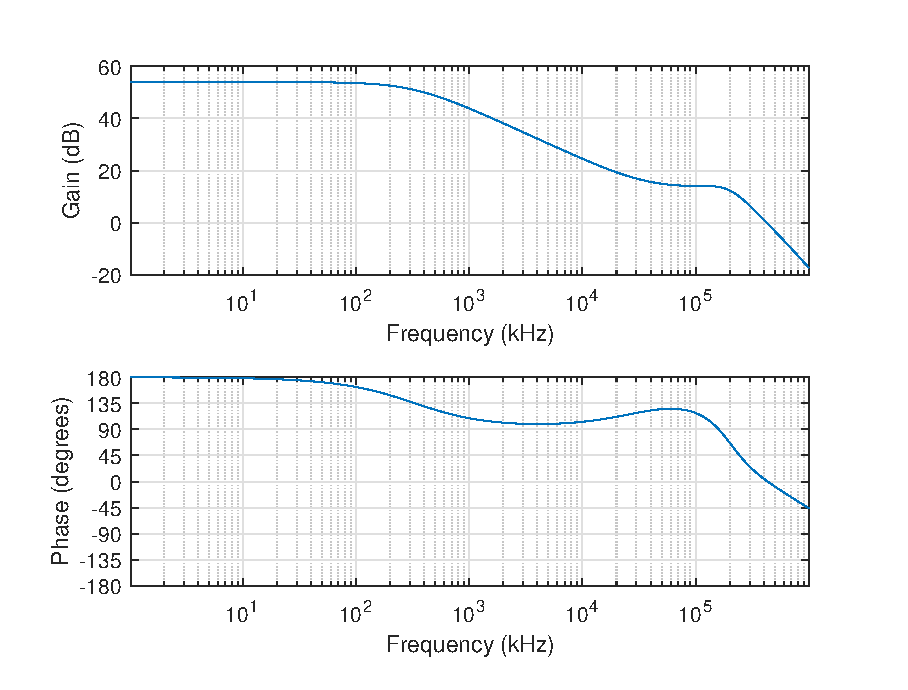
\includegraphics[width=\columnwidth]{figures/schematic/ac_dm.eps}
  \caption{AC differential mode frequency response of the amplifier with schematic models only.}
  \label{fig:sch_ac_dm}
\end{figure}

\begin{figure}[!htb]
  \centering
  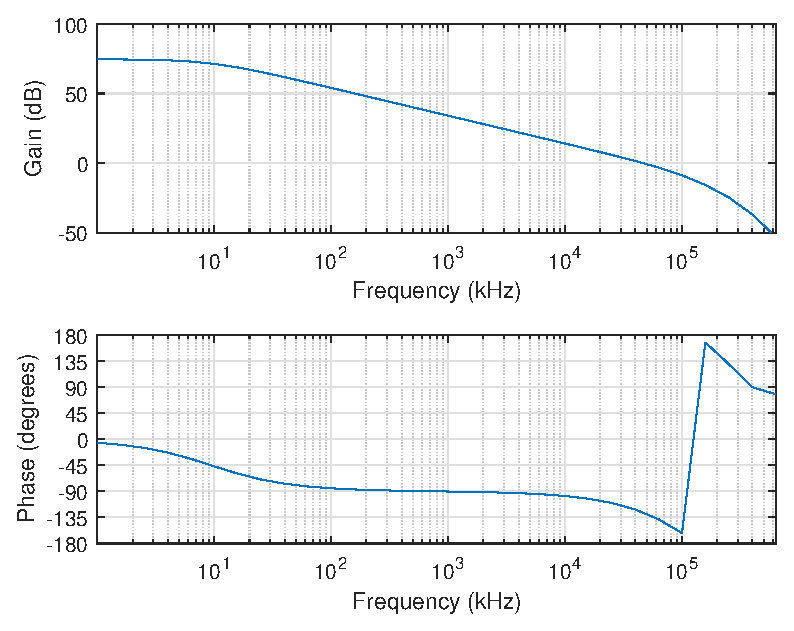
\includegraphics[width=\columnwidth]{figures/layout/ac_dm.eps}
  \caption{AC differential mode frequency response of the amplifier with layout parasitics extracted.}
  \label{fig:lay_ac_dm}
\end{figure}

Next, we measured the AC noise of the amplifier using the same setup. Using $V_d$ as our noise source, we obtained the output-referred spectral noise density shown in \Cref{fig:sch_ac_noise,fig:lay_ac_noise}. The noise was measured from $\SI{10}{\hertz}$ to $\SI{1}{\mega\hertz}$, with the RMS value over this bandwidth calculated to be $\SI{273}{\milli\volt}$ for the schematic simulation and $\SI{263}{\milli\volt}$ for the layout parasitics simulation. This slight difference is expected since the gain and bandwidth of the laid out amplifier are slightly lower.
In addition, we measured the input-referred spot noise at $\SI{1}{\mega\hertz}$, and found $\SI{36.9}{\nano\volt\per\sqrt{\hertz}}$ for the schematic simulation and $\SI{37.0}{\nano\volt\per\sqrt{\hertz}}$ for the layout parasitics simulation. Both of these satisfy the upper limit of $\SI{100}{\nano\volt\per\sqrt{\hertz}}$ given in the specifications, with no significant difference between the two.

\begin{figure}[!htb]
  \centering
  \includegraphics[width=\columnwidth]{figures/schematic/ac_noise.eps}
  \caption{Output-referred AC noise of the amplifier with schematic models only.}
  \label{fig:sch_ac_noise}
\end{figure}

\begin{figure}[!htb]
  \centering
  \includegraphics[width=\columnwidth]{figures/layout/ac_noise.eps}
  \caption{Output-referred AC noise of the amplifier with layout parasitics extracted.}
  \label{fig:lay_ac_noise}
\end{figure}

\section{Transient Analysis}

We then measured the closed loop transient behaviour of the amplifier using the setup shown in \Cref{fig:closed-loop-setup}, where the $\SI{1.2}{\volt}$ supply has been omitted for clarity.

\begin{figure}[!htb]
  \centering
  \includegraphics[width=\columnwidth]{schematics/closed-loop-setup.pdf}
  \caption{A schematic of the setup used for taking closed loop measurements of the amplifier.}
  \label{fig:closed-loop-setup}
\end{figure}

First, we input a fast $\SI{100}{\milli\volt}$ pulse to the circuit, starting at a DC bias point of $\SI{0.5}{\volt}$. The resulting output is shown in \Cref{fig:sch_tran_step,fig:lay_tran_step}. From these graphs, we can measure the rise time as $\SI{5.56}{\nano\second}$ for the schematic simulation and $\SI{5.77}{\nano\second}$ for the layout parasitics simulation. In addition, we can measure the settling time as $\SI{7.99}{\nano\second}$ for the schematic simulation and $\SI{13.8}{\nano\second}$ for the layout parasitics simulation. Here, we can see that the layout parasitics do have an effect on the step response of the amplifier, slightly degrading its rise and settling times.

\begin{figure}[!htb]
  \centering
  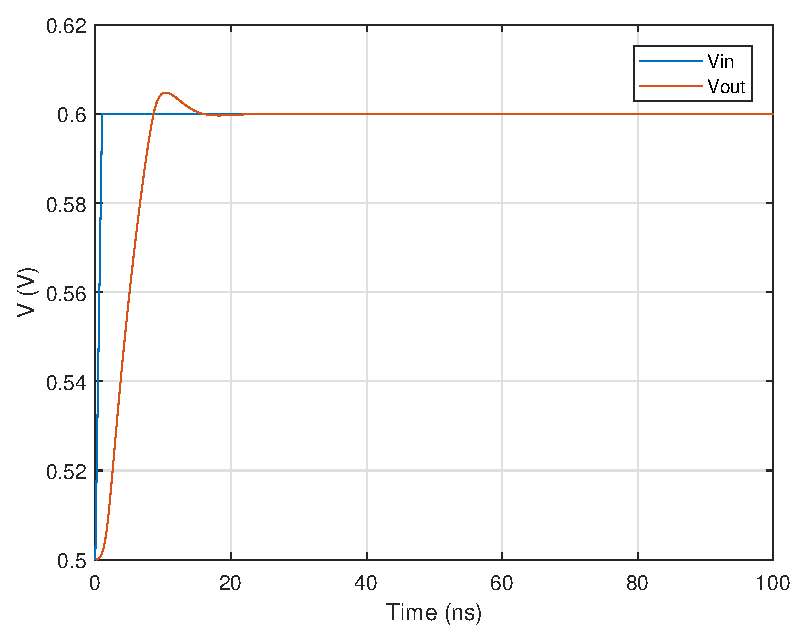
\includegraphics[width=\columnwidth]{figures/schematic/tran_step.eps}
  \caption{Transient step response of the amplifier with schematic models only.}
  \label{fig:sch_tran_step}
\end{figure}

\begin{figure}[!htb]
  \centering
  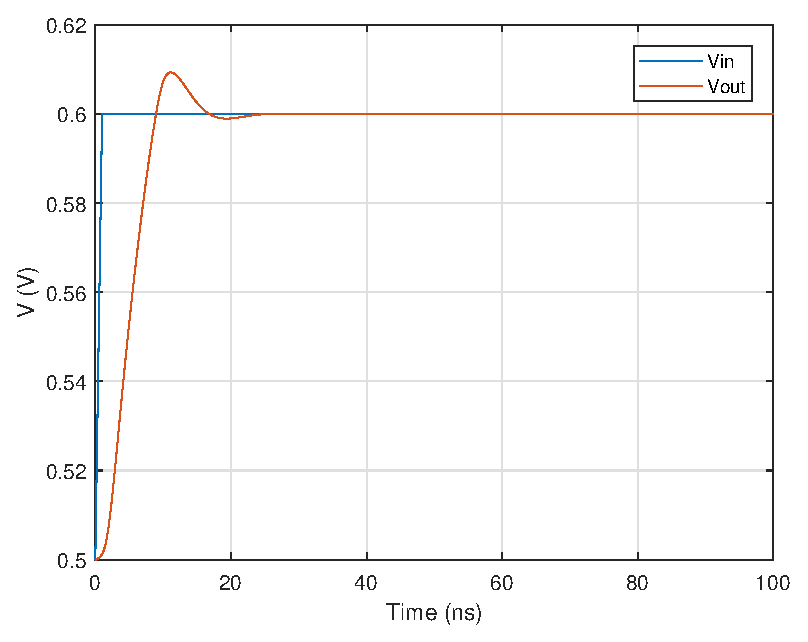
\includegraphics[width=\columnwidth]{figures/layout/tran_step.eps}
  \caption{Transient step response of the amplifier with layout parasitics extracted.}
  \label{fig:lay_tran_step}
\end{figure}

Next, we measured the distortion present when we input a $\SI{0.6}{\volt}$ peak-peak sine wave centered around the common mode point of $\SI{0.5}{\volt}$. This corresponds to a swing of half the supply range. The resulting output is shown in \Cref{fig:sch_tran_3m,fig:lay_tran_3m}. From these figures, we can measure the total harmonic distortion as $\SI{0.028}{\percent}$ for the schematic simulation and $\SI{0.053}{\percent}$ for the layout parasitics simulation. Thus, we have exceeded the specification of $\SI{0.2}{\percent}$ distortion at a swing equal to half the supply range for both cases. Therefore, the amplifier meets all the requirements, both with the schematic models only and with the layout parasitics extracted.

\begin{figure}[!htb]
  \centering
  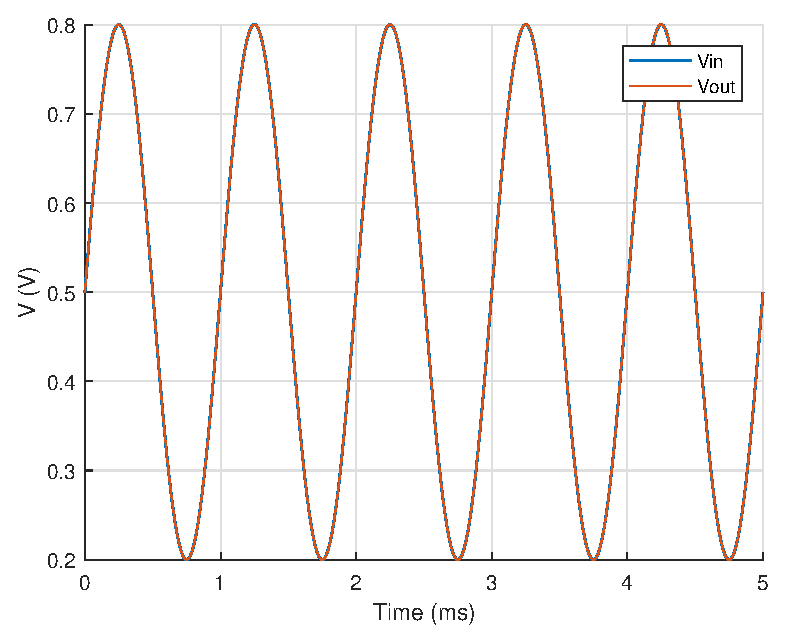
\includegraphics[width=\columnwidth]{figures/schematic/tran_3m.eps}
  \caption{Transient response of the amplifier with schematic models only to a $\SI{1}{\kilo\hertz}$, $\SI{300}{\milli\volt}$ amplitude sine wave input.}
  \label{fig:sch_tran_3m}
\end{figure}

\begin{figure}[!htb]
  \centering
  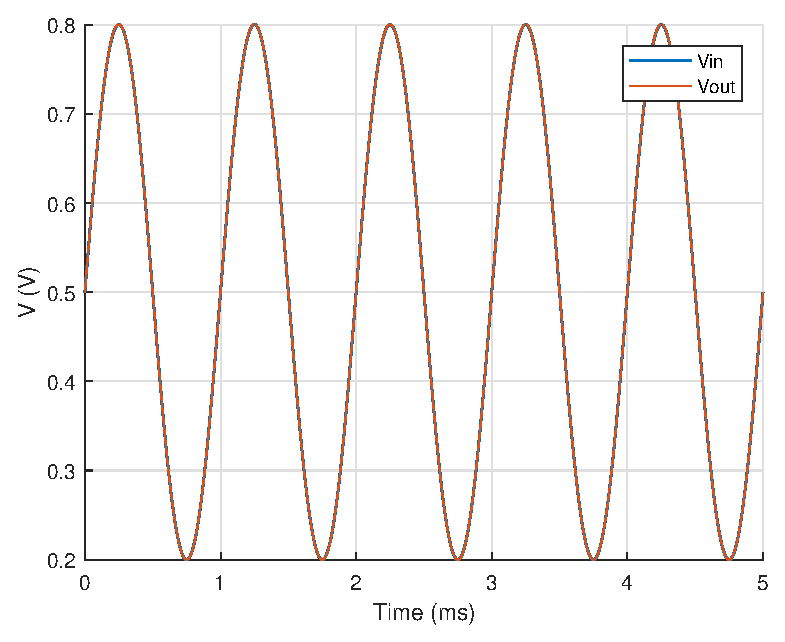
\includegraphics[width=\columnwidth]{figures/layout/tran_3m.eps}
  \caption{Transient response of the amplifier with layout parasitics extracted to a $\SI{1}{\kilo\hertz}$, $\SI{300}{\milli\volt}$ amplitude sine wave input.}
  \label{fig:lay_tran_3m}
\end{figure}

Finally, we measured the maximum input/output swing in the unity-gain configuration. To this end, we input a $\SI{1.6}{\volt}$ peak-peak, $\SI{1}{\kilo\hertz}$ sine wave centered around a DC bias point of $\SI{0.5}{\volt}$ and observed the output. The result is shown in \Cref{fig:sch_tran_8m,fig:lay_tran_8m}. These graphs shows a maximum input/output swing of $\SI{0.00}{\volt}$ to $\SI{1.00}{\volt}$ for the schematic simulation and $\SI{0.00}{\volt}$ to $\SI{1.05}{\volt}$ for the layout parasitics simulation. Again, we find no significant difference in the properties of the amplifier with and without layout parasitics.

\begin{figure}[!htb]
  \centering
  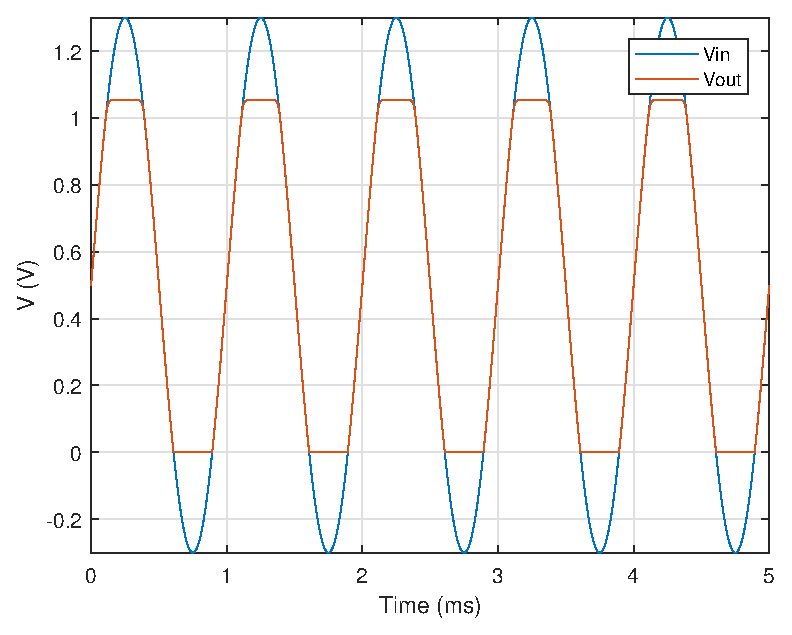
\includegraphics[width=\columnwidth]{figures/schematic/tran_8m.eps}
  \caption{Transient response of the amplifier with schematic models only to a large $\SI{1}{\kilo\hertz}$ sine wave input.}
  \label{fig:sch_tran_8m}
\end{figure}

\begin{figure}[!htb]
  \centering
  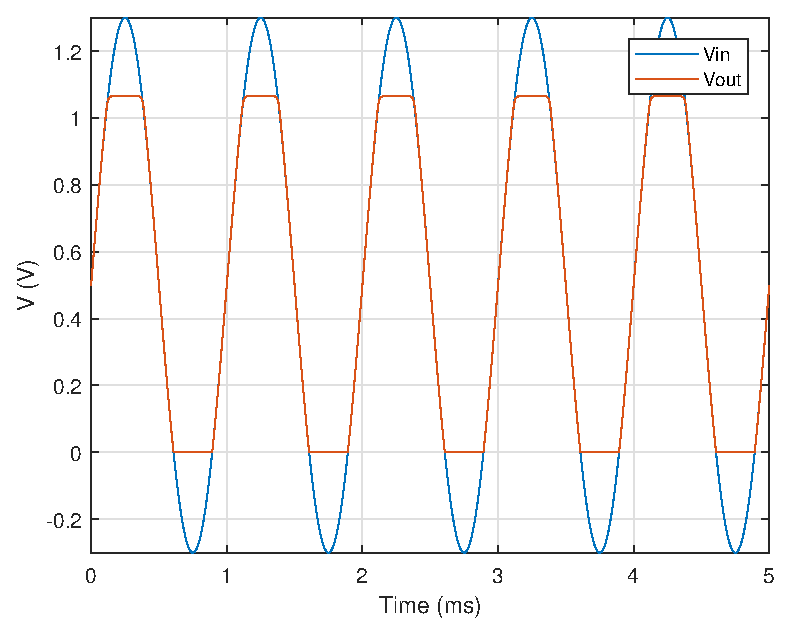
\includegraphics[width=\columnwidth]{figures/layout/tran_8m.eps}
  \caption{Transient response of the amplifier with layout parasitics extracted to a large $\SI{1}{\kilo\hertz}$ sine wave input.}
  \label{fig:lay_tran_8m}
\end{figure}

\section{Conclusions}

In conclusion, we performed the layout for a modified version of the amplifier we designed in Assignment \#2 and compared its performance when using just the schematic models with its performance when simulating the layout parasitics. We found no significant difference, with the amplifier still meeting all of its specifications, including a DC gain greater than $\SI{60}{\deci\bel}$, poles at approximately $\SI{10}{\kilo\hertz}$ and $\SI{100}{\mega\hertz}$, low distortion when swinging at half the supply range, low input-referred noise, and a static power dissipation of less than $\SI{200}{\micro\watt}$.

\bibliographystyle{IEEEtran}
\bibliography{IEEEabrv,references}

\end{document}
